\documentclass[english,a4paper,oneside,9pt]{extarticle}
%\documentclass[english,a4paper,twoside,9pt]{extarticle}
% Author: 
%
%	Oliver Sheridan-Methven, November 2017.
%	
% Description:
%
%	A collection of extremely useful packages 
%	which have been accumulated over a long time,
%	all of which combine to make very nice LaTeX
%	documents. 



\usepackage{adjustbox} % Nice alternative to minipage.
\usepackage{afterpage} % To give the title page its own geometry.
\usepackage{amsmath} % Nice maths symbols.
\usepackage{amssymb} % Nice variable symbols.
\usepackage{array} % Allow for custom column widths in tables.
\usepackage{ltablex} % For long tables spanning multiple pages. % Must be before ARYDSHLN package!
\keepXColumns % Keeps the X column
\usepackage{arydshln} % Dashed lines using \hdashline \cdashline
\usepackage{bbm} % Gives Blackboard fonts.
\usepackage{blindtext} % Generates dummy maths. cf. lipsum.
\usepackage{calc} % Calculates widths of words. 
\usepackage{chngcntr} % Changing counters, e.g. with footnotes.
\usepackage[nostamp]{draftwatermark} % Gives a draft overlay. Use options [nostamp] or [final].
\usepackage{emptypage} % Empty pages have no headers and footers.
\usepackage{enumitem} % Nice listing options in itemize and enumerate.
\usepackage{esdiff} % Gives nice differential operators.
\usepackage{etoolbox} % For defining conditionals. 
\usepackage{fancyhdr} % Nice headers.
\usepackage{float} % Nice figure placement.
\usepackage[T1]{fontenc} % Nice range of text characters and accents.
\usepackage[bottom]{footmisc} % Nice footnote formatting.
\usepackage{graphicx} % Include figures.
\usepackage[notquote]{hanging} % For indenting later lines in a paragraph. USE the 'noquote' option else the `'` is overwritten, and breaks in maths mode!
\usepackage{ifoddpage} % Checks for odd or even page.
\usepackage[geometry]{ifsym} % Useful symbols.
\usepackage{imakeidx} % Makes the index.
\usepackage{indentfirst} % Indents the first paragraph.
\usepackage{letltxmacro} % For defining a nice SQRT symbol.
\usepackage{lipsum} % Useful for adding jargon.
\usepackage{listings} % The listings package for code.
\usepackage{marginnote} % For nice margin notes.
\usepackage{mathtools} % Gives the colon equals symbol.
\usepackage[framed,numbered,autolinebreaks,useliterate]{mcode} % Inports Listings package ideal for MATLAB.
\usepackage[framemethod=tikz]{mdframed} % Gives nices boxed and sidesrules.
\usepackage{multirow} % Nice table cells spanning many rows.
\usepackage{multicol} % If I want to use multiple columns.
\usepackage[numbers, sort&compress]{natbib} % Nice references.
\usepackage{sansmath} % Gives a changing math font. %% Must be before newpxtext/newpxmath ! %%
\usepackage{newpxtext} % Gives Palatino and Helvetica fonts.
\usepackage{newpxmath} % Gives Palatino and Helvetica fonts in maths. 
\usepackage{bm} % Bold math symbols. %% Needs to be loaded after newpxtext/math. %%
\usepackage{nicefrac} % Gives nice fractions for superscripts.
\usepackage{nomencl} % Gives a symbol nomenclature. 
\usepackage[super]{nth} % Gives nice ordinal superscripts, eg 1st, 2nd, etc.
\usepackage{parskip} % Gives nicer indenting.
\usepackage{physics} % Nice partial derivatives and BRAKET notation.
\usepackage{ragged2e} % For nice allignment.
%\usepackage[norefs]{refcheck} % Can show any unused references.
\usepackage{romannum} % Nice typing for roman numerals.
\usepackage{setspace} % Ideal for increasing line spacing. E.g.  \doublespacing
\usepackage{siunitx} % Nice formating of units.
\usepackage{sidenotes} % Nice margin figures and margin tables. 
\usepackage{subcaption} % Side by side figures.
\usepackage[textsize=small]{todonotes} % A nice TODO list. [disable] to supress.
\usepackage{tikz} % Nice diagrams.
\usepackage{titling} % Access title variables. 
\usepackage{titlesec} % Nice section title colouring options.
\usepackage[nottoc]{tocbibind} % Gives nices Table of Contents
\usepackage{xcolor} % This is useful for making greyed table cells, nice for headers. Known preamble placement issues.
\usepackage{xifthen}% Provides \isempty test.
\usepackage{xparse} % Gives \NewDocumentEnvironment which has nice optional argument handling.
\usepackage{xspace} % Gives nice spacing for commands.
%%%% Generally HYPERREF should be imported last. %%%%
\usepackage[colorlinks=true,linkcolor=black,urlcolor=black,citecolor=black,anchorcolor=black]{hyperref} % Colour links.
%%%% Should be loaded after hyperref. %%%%
\usepackage{cleveref} % Gives smart referencing. %% After Hyperref
\usepackage[margin=10pt,font=small, textfont=bf,labelfont=bf,labelsep=endash]{caption} % Caption figures and tables nicely. %% After cleveref.
\usepackage[left=60mm,right=26mm,top=30mm,bottom=29mm, heightrounded, marginparwidth=41mm, marginparsep=8mm, headsep=10mm]{geometry} % Use nice margins. Does give a small change in the default page margins. 

\makeatletter
\if@twoside % commands below work only for twoside option of \documentclass
\newgeometry{left=26mm,right=60mm,top=30mm,bottom=29mm, heightrounded, marginparwidth=41mm, marginparsep=8mm, headsep=10mm}
\fi
\makeatother

% Ensures subsubsections are numbered.
\setcounter{secnumdepth}{3}

% Making an index. 
\makeindex

% Making a nomenclature. 
\makenomenclature
% The column width for any nomenclature. 
\setlength\nomlabelwidth{0.2\linewidth}

% Set the table of content depth to only subsections. 
\setcounter{tocdepth}{2}

% Supressing bad box warnings
%\hbadness=10000 

% Where to search for figures. 
\graphicspath{{../../figures/}{../../figures/logos/}}

% Present the references in the order they are used.
\bibliographystyle{unsrtnat}
% Reduce spacing between references. 
\setlength{\bibsep}{0pt plus 0.3ex}

% Listing -> Code in environment labels.
\renewcommand{\lstlistingname}{Code}
\crefname{listing}{code}{codes}
\Crefname{listing}{Code}{Codes}
\lstset{
    numbers=left, 
    basicstyle=\ttfamily\footnotesize,
    frame=single, % adds a frame around the code
    xleftmargin=20.4pt,
    xrightmargin=3.4pt,
    %	numbersep=3mm,
}
\newfloat{lstfloat}{htbp}{lop} % environment for placing lisings in to make them float. 

% Nice paragraph indents.
\setlength{\parindent}{0mm}

% Giving the references the right title.
\renewcommand{\bibname}{References}
\renewcommand{\listfigurename}{List of figures}
\renewcommand{\listtablename}{List of tables}

% Removes most hyphenation.
\tolerance=1
\emergencystretch=\maxdimen
\hyphenpenalty=10000
\hbadness=10000

% To change the spacing in lists:
%\setlist{noitemsep} % or \setlist{noitemsep} to leave space around whole list
% or
\setenumerate{itemsep=-0.2em,topsep=0.5em} % Seems to look nice.

% Custom column widths using C{2cm}, L, R, etc.
\newcolumntype{L}[1]{>{\raggedright\let\newline\\\arraybackslash\hspace{0pt}}m{#1}}
\newcolumntype{C}[1]{>{\centering\let\newline\\\arraybackslash\hspace{0pt}}m{#1}}
\newcolumntype{R}[1]{>{\raggedleft\let\newline\\\arraybackslash\hspace{0pt}}m{#1}}

% Gives a nice column separation in multicolumn mode.
\setlength{\columnsep}{5mm}

% Figure environment for use in multicolumn. To put in captions use \captionof{figure}{content of caption}.
\newenvironment{Figure}
{\par\medskip\noindent\minipage{\linewidth}}
{\endminipage\par\medskip}

% Gives the nice SQRT symbol.
\makeatletter
\let\oldr@@t\r@@t
\def\r@@t#1#2{%
    \setbox0=\hbox{$\oldr@@t#1{#2\,}$}\dimen0=\ht0
    \advance\dimen0-0.2\ht0
    \setbox2=\hbox{\vrule height\ht0 depth -\dimen0}%
    {\box0\lower0.4pt\box2}}
\LetLtxMacro{\oldsqrt}{\sqrt}
\renewcommand*{\sqrt}[2][\ ]{\oldsqrt[#1]{#2}}
\makeatother

% Some common math operators which need their own typesetting.
\DeclareMathOperator{\sign}{sign}
\DeclareMathOperator*{\argmin}{argmin}
\DeclareMathOperator*{\argmax}{argmax}

% Number equations down to the subection level, e.g. 1.2.3 is the third equation in
% subsection 2 of section 1.
%\numberwithin{equation}{section}
\newcommand*\tageq{\refstepcounter{equation}\tag{\theequation}}

% This makes the footnote counter reset in each section.
\counterwithin*{footnote}{section}

% Nice spacing in the first row of a table
\newcommand{\firstrowspacing}{\rule{0pt}{2.6ex}}
% For a more open look in tables.
\setlength\extrarowheight{3pt} 

% Some useful text commands.
\newcommand{\nag}{NAG\textsuperscript{\textregistered}\xspace}
\newcommand{\arm}{Arm\textsuperscript{\textregistered}\xspace}

% For nice headers and footers.
\pagestyle{fancy}
\fancyhf{}
\renewcommand{\headrulewidth}{0pt}
\newlength{\oneinch}
\setlength\oneinch{1in}
\newlength{\innermarginonesided}

\newtoggle{TWOSIDED}
\togglefalse{TWOSIDED}
\makeatletter
\if@twoside % commands below work only for twoside option of \documentclass
\toggletrue{TWOSIDED}
\fi
\makeatother

\setlength\innermarginonesided{\paperwidth-\textwidth-\oddsidemargin-1in}
\makeatletter
\if@twoside
\setlength\innermarginonesided{\evensidemargin+1in}
\fi
\makeatother


\definecolor{header1}{RGB}{253,252,204}
\definecolor{header2}{RGB}{204,236,255}
\definecolor{header3}{RGB}{37,141,255}
\definecolor{header4}{RGB}{0,117,246}
\definecolor{header5}{RGB}{0,73,154}
\fancyhead[RE]{%
    \begin{adjustbox}{left, minipage=0.9\paperwidth}
        \hspace*{-0.8\innermarginonesided}
        \begin{tikzpicture}[overlay]
        \fill[fill=header5, draw=header5, minimum height=8mm, minimum width=16.4cm,anchor=west] (0,-1.4em) rectangle (1.0\linewidth,1.5em);
        \fill[fill=header4, draw=header4, minimum height=8mm, minimum width=16.4cm,anchor=west] (0.7\linewidth,-1.4em) rectangle (\linewidth,1.5em);
        \fill[fill=header3, draw=header3, minimum height=8mm, minimum width=16.4cm,anchor=west] (0.8\linewidth,-1.4em) rectangle (\linewidth,1.5em);
        \fill[fill=header2, draw=header2, minimum height=8mm, minimum width=16.4cm,anchor=west] (0.85\linewidth,-1.4em) rectangle (\linewidth,1.5em);        
        \fill[fill=header1, draw=header1, minimum height=8mm, minimum width=16.4cm,anchor=east] (0.9\linewidth,-1.4em) rectangle (\linewidth,1.5em);
        \end{tikzpicture}%
\end{adjustbox}%
    }
\fancyhead[LO]{%
    \begin{adjustbox}{right, minipage=0.9\paperwidth}
        \hspace*{0.8\innermarginonesided}
        \begin{tikzpicture}[overlay]
        \fill[fill=header5, draw=header5, minimum height=8mm, minimum width=16.4cm,anchor=east] (0,-1.4em) rectangle (1.0\linewidth,1.5em);
        \fill[fill=header4, draw=header4, minimum height=8mm, minimum width=16.4cm,anchor=east] (0,-1.4em) rectangle (0.3\linewidth,1.5em);
        \fill[fill=header3, draw=header3, minimum height=8mm, minimum width=16.4cm,anchor=east] (0,-1.4em) rectangle (0.2\linewidth,1.5em);
        \fill[fill=header2, draw=header2, minimum height=8mm, minimum width=16.4cm,anchor=east] (0,-1.4em) rectangle (0.15\linewidth,1.5em);        
        \fill[fill=header1, draw=header1, minimum height=8mm, minimum width=16.4cm,anchor=east] (0,-1.4em) rectangle (0.1\linewidth,1.5em);
        \end{tikzpicture}%
\end{adjustbox}%
    }

\newcommand{\textoverline}[1]{$\overline{\mbox{#1}}$}
% The footers are specified but are not the same margin widths as the headers. 
\fancyfoot[LE]{\hspace*{-0.8\innermarginonesided}\begin{adjustbox}{left, minipage=0.9\paperwidth}
        \raggedright
        \color{cyan}\textoverline{\color{black}\underline{\hphantom{\ }\thepage
                \begin{minipage}[c]{0\linewidth}
                    \rule{0pt}{2.5ex}
                \end{minipage}
                \rule{0.9\linewidth}{0pt}\rule{0pt}{2.0ex}}}
    \end{adjustbox}
}
\fancyfoot[RO]{\hspace*{0.8\innermarginonesided}\begin{adjustbox}{right, minipage=0.9\paperwidth}
        \raggedleft
        \color{cyan}\textoverline{\color{black}\underline{
                \begin{minipage}[c]{0\linewidth}
                    \rule{0pt}{2.5ex}
                \end{minipage}
                \rule{0.9\linewidth}{0pt}\rule{0pt}{2.0ex}\thepage\hphantom{\ }}}
    \end{adjustbox}
}
\fancypagestyle{plain}{%
    \fancyhf{}%
    \renewcommand*{\headrulewidth}{0pt}%
}
\cfoot{}


% Make margin notes small
\renewcommand*{\marginfont}{\noindent \small}
%\IfBooleanTF{@twoside}{\reversemarginpar}{}% If I want a wider margin by the binding.
% Ensuring nice justification.
\renewcommand\raggedrightmarginnote{\sloppy}
\renewcommand\raggedleftmarginnote{\sloppy}

% Gives a nice quote environment.
\NewDocumentEnvironment{myquote}{O{}}{%
    \begin{center}
        \begin{minipage}{0.85\linewidth}
            \vspace{1ex}
            \centering \itshape \justifying}
        {%
            \ifthenelse{\isempty{#1}}{}{
                \begin{flushright}%The author/source.
                    \normalfont #1
            \end{flushright}}
            \vspace{1ex}
        \end{minipage}
    \end{center}
}

% Gives a nice siderule environment. e.g. \begin{siderules}
\newmdenv[topline=false,bottomline=false,rightline=false,skipabove=\topsep,skipbelow=\topsep]{siderules}

% For a numbered description. Use inside enumerate, \litem{Something} etc. 
\newcommand\litem[1]{\item{\textbf{\underline{\smash{{#1}}:}}}}

% Nice spacing in lists
%\setlist{listparindent=\parindent,parsep=1ex} 

% This aligns figures in the adjust box environment to the inner margin. For use with "myalignedfigure" (below).
\newcommand{\aligninner}{\ifoddpage \raggedright \else \raggedleft \fi}%

% Gives a nice aligned figure environment, where figures are flush to the inner margin overflowing off the outer margin first. Useful for very wide figures, or set of lots of sub figures. 
\NewDocumentEnvironment{myalignedfigure}{O{1.3} O{htb}}{% fractional_linewidth,  position
    \begin{figure}[#2]
        \checkoddpage
        \edef\whichside{\ifoddpage left\else right\fi}
        \begin{adjustbox}{\whichside, minipage=#1\linewidth}}
        {%
        \end{adjustbox}
    \end{figure}
}

% Gives a nice draft text.
\SetWatermarkScale{1}
\SetWatermarkLightness{0.9}

% The oxford comma from cref for multiple citations. 
\newcommand{\creflastconjunction}{, and\nobreakspace}

% Define the dummy sentence, an ancient palindrome.
\def\sator{Sator Arepo tenet opera rotas.\xspace}

% A command to print the sentence repeatedly.
% Argument #1 is the number of times to repeat it.
\newcount\loopcounter
\def\dummysentences#1{%
    \loopcounter = #1
    \loop
    \sator\ %
    \advance\loopcounter by -1
    \ifnum\loopcounter > 0
    \repeat%
}

% Oxford blue
\definecolor{oxfordblue}{RGB}{0, 33, 71}

% Ensuring side boxes have shadows. 
\usetikzlibrary{shadows} % For shadowed boxes.
\tikzset{every shadow/.style={opacity=1}} % Shadows given full opacity. 

% Temporary environment for the InFoMM side bubble. 
\NewDocumentEnvironment{mysidenote}{}{% verticle offset
    \noindent
    \begin{minipage}[t]{\linewidth}		\begin{mdframed}[roundcorner=5pt, linecolor=oxfordblue, linewidth=2pt, backgroundcolor=yellow!40, shadow=true,shadowcolor=black,shadowsize=6pt]\raggedright
        }
        {
        \end{mdframed}
    \end{minipage}
}

% The final command for an InFoMM margin bubble. 
\newcommand{\infommmarginnote}[2][0mm]{\marginnote{\large\sffamily{}\sansmath\begin{mysidenote}{#2}\end{mysidenote}}[{#1}]}

% Useful for drawing a page border. 
\usetikzlibrary{calc}

% Enable blind maths. 
\blindmathtrue

%InFoMM glossary
\NewDocumentEnvironment{infommitemize}{}{% verticle offset
    \noindent
    \begin{itemize}[label={\color{cyan}{$\blacksquare$}}]
    }
    {%
    \end{itemize}
}

\newcommand{\coverimage}[1][cover_image]{
    \newcommand{\thecoverimage}{#1}
}

% Nice colouring of section titles
\titleformat{\section}
{\color{oxfordblue}\normalfont\fontsize{16}{20}\selectfont\bfseries}
{\color{oxfordblue}\thesection}{1em}{\thesection.\hspace{1ex}}
\titleformat{\subsection}
{\color{cyan}\normalfont\Large\bfseries}
{\color{cyan}\thesection}{1em}{}
\titleformat{\subsubsection}
{\color{cyan}\normalfont\Large\bfseries}
{\color{cyan}\thesection}{1em}{}

% Shorten the spacing after section headings
\titlespacing\section{0pt}{12pt plus 4pt minus 2pt}{0pt plus 2pt minus 2pt}
\titlespacing\subsection{0pt}{12pt plus 4pt minus 2pt}{0pt plus 2pt minus 2pt}
\titlespacing\subsubsection{0pt}{12pt plus 4pt minus 2pt}{0pt plus 2pt minus 2pt}



% Remove section numbers in TOC. 
%\makeatletter
%\let\latexl@section\l@section
%\def\l@section#1#2{\begingroup\let\numberline\@gobble\latexl@section{#1}{#2}\endgroup}
%\makeatother
% Remove subsection numbers in TOC. 
\makeatletter
\let\latexl@subsection\l@subsection
\def\l@subsection#1#2{\begingroup\let\numberline\@gobble\latexl@subsection{\quad#1}{#2}\endgroup}
\makeatother





\title{Mini-project lay report}
\author{Oliver Sheridan-Methven}
\coverimage[cover_image] % Specify your own image using [].


\begin{document}

% The cover page is a designed to look best on A4 and is designed to be a
% "What you see is what you get".
\thispagestyle{empty} % 'gobble' pagestyle throws issues with nomencl package. 
\afterpage{
%\pagestyle{empty}
\newgeometry{left = 20mm, right = 20mm, top = 15mm, bottom = 10mm}

\newgeometry{left = 20mm, right = 20mm, top = 30mm, bottom = 30mm}
\pagestyle{empty}
\begin{tikzpicture}[remember picture, overlay]
\draw [line width=2mm, oxfordblue]
($ (current page.south west) + (8mm, 8mm) $)
rectangle
($ (current page.north east) + (-8mm, -8mm)$);
\node[anchor=north west, xshift=10mm, yshift=-10mm] at (current page.north west) {
\includegraphics[width=0.3\linewidth]{epsrc_logo}};
\node[anchor=north east, xshift=-10mm, yshift=-10mm] at (current page.north east) {
\includegraphics[width=0.3\linewidth]{infomm_logo_blue}};
\node[anchor=south west, xshift=10mm, yshift=10mm] at (current page.south west) {
\includegraphics[width=0.3\linewidth]{oxford_logo_blue_long}};
\node[anchor=south east, xshift=-10mm, yshift=10mm] at (current page.south east) {\includegraphics[width=0.4\linewidth]{\thecompanylogo}};
\end{tikzpicture}

\begin{center}
\vfill
{\fontsize{25}{28}\selectfont\color{oxfordblue}\textbf{EPSRC Centre for Doctoral Training in Industrially Focused Mathematical Modelling}}
\vfill
\begin{figure}[h]
\centering
\includegraphics[width=0.7\linewidth]{\thecoverimage}
\end{figure}
\vfill
{\fontsize{25}{28}\selectfont\color{oxfordblue}\textbf{\thetitle}}\\
\vfill
{\fontsize{20}{25}\selectfont\color{oxfordblue}\color{oxfordblue}\textbf{\theauthor}}
\vfill
\end{center}
\restoregeometry
}
\clearpage
	
% Table of contents page.
\afterpage{
	\titleformat{\section}
	{\color{oxfordblue}\normalfont\fontsize{16}{20}\selectfont\bfseries}
	{\color{black}\thesection}{1em}{}
\pagestyle{empty}
\newgeometry{left=110mm,right=20mm,top=30mm,bottom=29mm, heightrounded, marginparwidth=100mm, marginparsep=5mm}
\reversemarginpar
\noindent
\doublespacing
\begin{minipage}[t]{\linewidth}
\tableofcontents
\end{minipage} \\
\marginpar{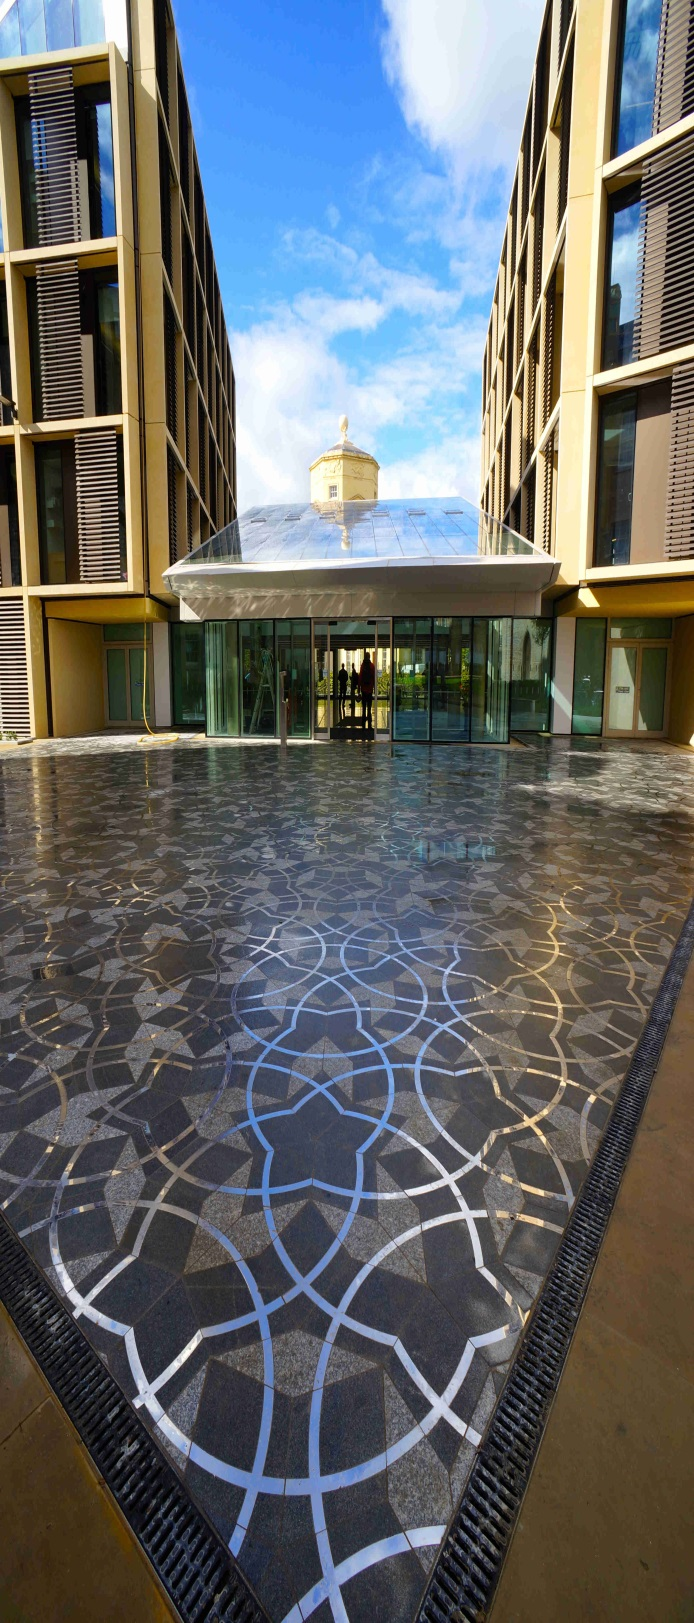
\includegraphics[width=\linewidth]{andrew_wiles_building}}
\clearpage
}

\cleardoublepage % Double page as page numbering starts at 1.
\setcounter{section}{0}
\pagenumbering{arabic}


% For proof reading
%\doublespacing

\section{Introduction}
\subsection{Background information}

\infommmarginnote{\dummysentences{3}}
\infommmarginnote[10em]{We can change the vertical spacing of these boxes using the optional command. (1em approximately corresponds to a line)}
\lipsum[2]

We can reference loads of useful stuff like \Cref{fig:harris_cartoon,fig:side_cartoon}, and also \Cref{tab:some_useful_values}.

\begin{table}[htb]
    \centering
    \begin{tabular}{llll}
    	Quantity        & Name      & Value                 & Units                                \\ \hline
    	Time            & Tenure    & 12                    & \si{\micro\second}                   \\
    	Length          & Height    & 1.82                  & \si{\centi\meter}                    \\
    	Planks constant & $ \hbar $ & $ 6.62\cdot10^{-32} $ & \si{\meter^2.\kilogram.\second^{-1}}
    \end{tabular}
    \caption{Some useful values.}
    \label{tab:some_useful_values}
\end{table}


\subsubsection{Very specific points}
\todo{In the margin I can mention something I need to do.}
\lipsum[75]
\todo[inline=true]{Incase I need to highlight something I need to do.}


It's all  about \marginnote{
	\begin{center}
		\begin{tabular}{lll}
			 & Value & Units \\ \hline
			c & $ 3\cdot10^{3} $ & \si{\meter.\second^{-1}} \\
			$ \hbar $ & $ 6.62\cdot10^{-32} $ & \si{\meter^2.\kilogram.\second^{-1}} \\
		\end{tabular}
	\end{center}
	\captionof{table}{Some physical constants which frequently come in handy for calculations, (although InFoMM students always non-dimensionalise).}
}
\begin{equation}
 \norm{\bm{l}}_\infty^4 = \pdv[4]{f}{\bm{g}}\coloneqq x^2 + y^2 = z^2.
\end{equation}

\subsubsection{Glossary of terms}

\begin{infommitemize}
	\litem{Cartoon} A brilliant sketch.
	\litem{Lay report} A smaller version of the technical report without all the maths.
	\litem{InFoMM} A great way to get a PhD and change the world. 
	\litem{Something a bit odd} \dummysentences{5}
\end{infommitemize}


\lipsum[1]

\subsubsection{An odd point}

\begin{figure}[htb]
\marginnote{
    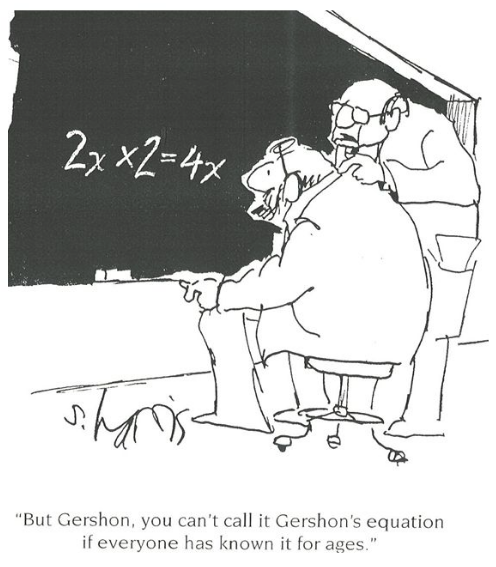
\includegraphics[width=\linewidth]{cover_image}
    \captionof{figure}{He is my favourite cartoonist.}
    \label{fig:side_cartoon}}
\centering
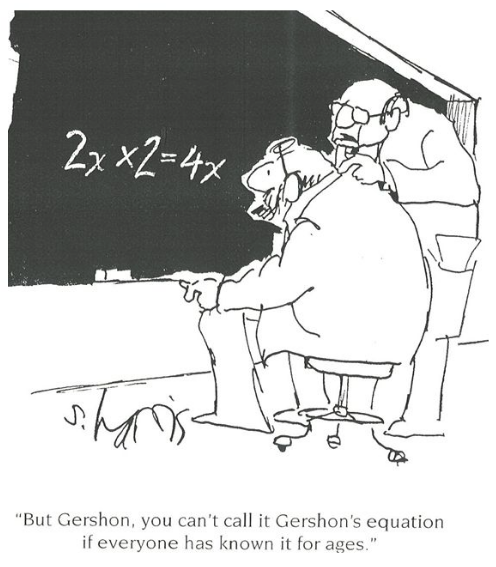
\includegraphics[width=0.7\linewidth]{cover_image}
\caption{A hilarious S.\,Harris cartoon. Here $ e = mc^2 $ or $ \bm{e = mc^2}$.}
\label{fig:harris_cartoon}
\end{figure} 

\lipsum[1]

\infommmarginnote[3mm]{I love these side bubbles! They're awesome and very helpful.
	$$ \int_{\mathbb{R}}^{\infty^+} f(z) \dd(z)  = 0
	$$}
\lipsum[1]


\section{Some crazy maths}

\Cref{code:example} is a nice example of using Python rather than Matlab.

\begin{lstfloat}[htb]
\begin{lstlisting}[language=Python, caption={[Example prime number generator]Some example python code, incase we wanted to show the company some awesome programming idea.}, label={code:example}, captionpos=b]
def prime_numbers():
	"""
	A prime number generator.
	:return: Int, prime number.
	"""
	x = 2
	primes = [x]
	yield x  # We the first prime number.
	while True:
		if x in primes:
			x += 1
		else:
			is_prime = True  
			for p in primes:
				if x % p == 0:
					is_prime = False  # The number is not prime.
					x += 1
					break  # We do not need further checks.
			if is_prime:
				primes.append(x)
				yield x
\end{lstlisting}
\end{lstfloat}

\blindmathpaper

\section{Discussion, conclusions \& recommendations}
\dummysentences{3}

For general quotes use:
\begin{myquote}[Caesar, head of the Roman empire.]
\lipsum[66]
\end{myquote}

While for the final company quote use:

[Insert name], [Job title + company] said: ``\emph{\dummysentences{5}}''

% Add the bibliography.
\begin{small}
%	\nocite{*} % Publishes any unused references.
\bibliography{references}
\end{small}

\section{COMMENTS ON THE REPORT}
For the \textbf{final} editing:
\begin{itemize}
    \item Ensure the side bubbles are correctly centred and don't spill over any pages. 
    \item Ensure there are no dangling headers (This might require inserting a \verb|\clearpage| command.)
\end{itemize}
\clearpage
\end{document}
